% Unicode build: XeLaTeX/Tectonic; LuaLaTeX is also supported.
% Official ACL style files are unchanged. Main content: sections 1--6.
\documentclass[11pt]{article}
\usepackage[preprint]{acl}
\usepackage{microtype}
\usepackage[english,bidi=default]{babel}
\babelfont{rm}{TeXGyreTermesX}
\usepackage{fontspec}
\usepackage{iftex}
\ifLuaTeX
  \newfontfamily\hifont[Path=fonts/,Extension=.ttf,UprightFont=NotoSansDevanagari-Regular,BoldFont=NotoSansDevanagari-Bold,Script=Devanagari,Renderer=HarfBuzz]{NotoSansDevanagari}
  \newfontfamily\gufont[Path=fonts/,Extension=.ttf,UprightFont=NotoSansGujarati-Regular,BoldFont=NotoSansGujarati-Bold,Script=Gujarati,Renderer=HarfBuzz]{NotoSansGujarati}
\else
  \newfontfamily\hifont[Path=fonts/,Extension=.ttf,UprightFont=NotoSansDevanagari-Regular,BoldFont=NotoSansDevanagari-Bold,Script=Devanagari]{NotoSansDevanagari}
  \newfontfamily\gufont[Path=fonts/,Extension=.ttf,UprightFont=NotoSansGujarati-Regular,BoldFont=NotoSansGujarati-Bold,Script=Gujarati]{NotoSansGujarati}
\fi
% Generated from native strings in the editable section/figure/table sources.
% UTF-16BE ActualText prevents visual-order extraction of Indic vowel signs.
\expandafter\def\csname aacunicode@थका हुआ\endcsname{09250915093E0020093909410906}
\expandafter\def\csname aacunicode@दमलेला\endcsname{0926092E093209470932093E}
\expandafter\def\csname aacunicode@नको\endcsname{09280915094B}
\expandafter\def\csname aacunicode@नहीं\endcsname{0928093909400902}
\expandafter\def\csname aacunicode@नहीं + खुश\endcsname{09280939094009020020002B0020091609410936}
\expandafter\def\csname aacunicode@नहीं + पिज़्ज़ा\endcsname{09280939094009020020002B0020092A093F091C093C094D091C093C093E}
\expandafter\def\csname aacunicode@नाही\endcsname{0928093E09390940}
\expandafter\def\csname aacunicode@नाही + आनंदी\endcsname{0928093E093909400020002B002009060928090209260940}
\expandafter\def\csname aacunicode@नाही + पिझ्झा\endcsname{0928093E093909400020002B0020092A093F091D094D091D093E}
\expandafter\def\csname aacunicode@पाणी\endcsname{092A093E09230940}
\expandafter\def\csname aacunicode@पानी\endcsname{092A093E09280940}
\expandafter\def\csname aacunicode@पिज़्ज़ा, मुझे चाहिए।\endcsname{092A093F091C093C094D091C093C093E002C0020092E0941091D09470020091A093E0939093F090F0964}
\expandafter\def\csname aacunicode@पिणे + पाणी\endcsname{092A093F092309470020002B0020092A093E09230940}
\expandafter\def\csname aacunicode@पीना + पानी\endcsname{092A09400928093E0020002B0020092A093E09280940}
\expandafter\def\csname aacunicode@पीना, मुझे पानी चाहिए।\endcsname{092A09400928093E002C0020092E0941091D09470020092A093E092809400020091A093E0939093F090F0964}
\expandafter\def\csname aacunicode@फ़ोन करना + माँ\endcsname{092B093C094B09280020091509300928093E0020002B0020092E093E0901}
\expandafter\def\csname aacunicode@फोन करणे + आई\endcsname{092B094B0928002009150930092309470020002B002009060908}
\expandafter\def\csname aacunicode@मला आईला फोन करण्याची इच्छा आहे.\endcsname{092E0932093E0020090609080932093E0020092B094B09280020091509300923094D092F093E091A094000200907091A094D091B093E0020090609390947002E}
\expandafter\def\csname aacunicode@मला दमलेला हवे आहे.\endcsname{092E0932093E00200926092E093209470932093E00200939093509470020090609390947002E}
\expandafter\def\csname aacunicode@मला पाणी पिण्याची इच्छा आहे.\endcsname{092E0932093E0020092A093E092309400020092A093F0923094D092F093E091A094000200907091A094D091B093E0020090609390947002E}
\expandafter\def\csname aacunicode@मला पाणी हवे आहे.\endcsname{092E0932093E0020092A093E0923094000200939093509470020090609390947002E}
\expandafter\def\csname aacunicode@मला पिझ्झा नको आहे.\endcsname{092E0932093E0020092A093F091D094D091D093E002009280915094B0020090609390947002E}
\expandafter\def\csname aacunicode@मला पिझ्झा हवे आहे.\endcsname{092E0932093E0020092A093F091D094D091D093E00200939093509470020090609390947002E}
\expandafter\def\csname aacunicode@माँ, मुझे फ़ोन करना हूँ, मुझे चाहिए।\endcsname{092E093E0901002C0020092E0941091D09470020092B093C094B09280020091509300928093E0020093909420901002C0020092E0941091D09470020091A093E0939093F090F0964}
\expandafter\def\csname aacunicode@मी आनंदी नाही.\endcsname{092E094000200906092809020926094000200928093E09390940002E}
\expandafter\def\csname aacunicode@मी दमलेला सांगत आहे.\endcsname{092E094000200926092E093209470932093E00200938093E0902091709240020090609390947002E}
\expandafter\def\csname aacunicode@मुझे गुस्सा चाहिए।\endcsname{092E0941091D09470020091709410938094D0938093E0020091A093E0939093F090F0964}
\expandafter\def\csname aacunicode@मुझे पानी चाहिए।\endcsname{092E0941091D09470020092A093E092809400020091A093E0939093F090F0964}
\expandafter\def\csname aacunicode@मुझे पिज़्ज़ा नहीं चाहिए।\endcsname{092E0941091D09470020092A093F091C093C094D091C093C093E002009280939094009020020091A093E0939093F090F0964}
\expandafter\def\csname aacunicode@मैं खुश नहीं हूँ।\endcsname{092E0948090200200916094109360020092809390940090200200939094209010964}
\expandafter\def\csname aacunicode@मैं थका हुआ हूँ।\endcsname{092E09480902002009250915093E002009390941090600200939094209010964}
\expandafter\def\csname aacunicode@हवे आहे\endcsname{0939093509470020090609390947}
\expandafter\def\csname aacunicode@થાકેલું\endcsname{0AA50ABE0A950AC70AB20AC10A82}
\expandafter\def\csname aacunicode@નથી\endcsname{0AA80AA50AC0}
\expandafter\def\csname aacunicode@ના + ખુશ\endcsname{0AA80ABE0020002B00200A960AC10AB6}
\expandafter\def\csname aacunicode@ના + પિઝા\endcsname{0AA80ABE0020002B00200AAA0ABF0A9D0ABE}
\expandafter\def\csname aacunicode@નાક\endcsname{0AA80ABE0A95}
\expandafter\def\csname aacunicode@પાણી\endcsname{0AAA0ABE0AA30AC0}
\expandafter\def\csname aacunicode@પીવું + પાણી\endcsname{0AAA0AC00AB50AC10A820020002B00200AAA0ABE0AA30AC0}
\expandafter\def\csname aacunicode@ફોન કરવો + માતા\endcsname{0AAB0ACB0AA800200A950AB00AB50ACB0020002B00200AAE0ABE0AA40ABE}
\expandafter\def\csname aacunicode@મને પાણી જોઈએ છે.\endcsname{0AAE0AA80AC700200AAA0ABE0AA30AC000200A9C0ACB0A880A8F00200A9B0AC7002E}
\expandafter\def\csname aacunicode@મને પાણી પીવાનું મન છે.\endcsname{0AAE0AA80AC700200AAA0ABE0AA30AC000200AAA0AC00AB50ABE0AA80AC10A8200200AAE0AA800200A9B0AC7002E}
\expandafter\def\csname aacunicode@મને પિઝા નથી જોઈતું.\endcsname{0AAE0AA80AC700200AAA0ABF0A9D0ABE00200AA80AA50AC000200A9C0ACB0A880AA40AC10A82002E}
\expandafter\def\csname aacunicode@મને માતાને ફોન કરવાનું મન છે.\endcsname{0AAE0AA80AC700200AAE0ABE0AA40ABE0AA80AC700200AAB0ACB0AA800200A950AB00AB50ABE0AA80AC10A8200200AAE0AA800200A9B0AC7002E}
\expandafter\def\csname aacunicode@હું ખરાબ છું.\endcsname{0AB90AC10A8200200A960AB00ABE0AAC00200A9B0AC10A82002E}
\expandafter\def\csname aacunicode@હું ખુશ નથી.\endcsname{0AB90AC10A8200200A960AC10AB600200AA80AA50AC0002E}
\expandafter\def\csname aacunicode@હું થાકેલું છું.\endcsname{0AB90AC10A8200200AA50ABE0A950AC70AB20AC10A8200200A9B0AC10A82002E}

% Native glyph shaping and exact Unicode extraction are both preserved.
\ifXeTeX
  \newcommand{\aacactualstart}[1]{\special{pdf:code /Span << /ActualText <FEFF\csname aacunicode@#1\endcsname> >> BDC}}
  \newcommand{\aacactualend}{\special{pdf:code EMC}}
\else
  \newcommand{\aacactualstart}[1]{}
  \newcommand{\aacactualend}{}
\fi
\DeclareRobustCommand{\hi}[1]{{\hifont\upshape\aacactualstart{#1}#1\aacactualend}}
\DeclareRobustCommand{\gu}[1]{{\gufont\upshape\aacactualstart{#1}#1\aacactualend}}
\usepackage{booktabs,graphicx,amsmath,array,xcolor,enumitem,float,tikz}
\usetikzlibrary{arrows.meta,positioning}
\setlist{nosep,leftmargin=*}
\definecolor{exampleblue}{HTML}{075985}
\definecolor{examplegreen}{HTML}{166534}
\definecolor{errorred}{HTML}{B91C1C}
\definecolor{panelgray}{HTML}{F2F5F7}
\newcommand{\good}[1]{\textcolor{exampleblue}{#1}}
\newcommand{\kept}[1]{\textcolor{examplegreen}{#1}}
\newcommand{\bad}[1]{\textcolor{errorred}{#1}}
\newcommand{\lang}[1]{\textbf{\textit{#1}}}
\newcommand{\sys}{Indic AAC Studio}
\newcommand{\model}{Qwen2.5-0.5B-Instruct}
\newcolumntype{L}[1]{>{\raggedright\arraybackslash}p{#1}}
\setcounter{topnumber}{3}\setcounter{totalnumber}{5}\setcounter{dbltopnumber}{3}
\renewcommand{\topfraction}{0.9}\renewcommand{\textfraction}{0.08}
\renewcommand{\floatpagefraction}{0.75}\renewcommand{\dblfloatpagefraction}{0.75}
\title{Indic AAC Studio: Concept-Gated Symbol-to-Sentence Generation\\
for English, Hindi, Gujarati, and Marathi}
\setlength\titlebox{13\baselineskip}
\author{Ravindrakumar M. Purohit \\
  Speech Research Lab \\
  Dhirubhai Ambani University (DA-IICT) \\
  Gandhinagar, India
  \And
  Jaydeep Parmar \\
  Pandit Deendayal Energy \\
  University (PDEU) \\
  Gandhinagar, India
  \AND
  Hemant A. Patil \\
  Speech Research Lab, Dhirubhai Ambani University (DA-IICT), Gandhinagar, India}
\begin{document}
\maketitle
\begin{abstract}
Expanding a symbol selection into a sentence for augmentative and alternative communication (AAC) must preserve the user's message.
A language model may instead replace a concept, reverse negation, or introduce an unselected need.
We present \sys{}, a four-language prototype that checks candidate concepts, polarity, and communicative act, then retries or uses a template when a candidate fails.
On 175 archived scenarios, the complete gate, retry, and fallback policy raises lexical success from 65/175 to 97/175 with actual web-client inputs, retains 215/215 required concept instances, and produces no detected polarity error.
The matched template scores 118/175, so this evidence supports a safeguard against cascade errors rather than a phrasing advantage over templates.
An audit motivates explicit act selection, multilingual checks, and checked fallbacks; both the revised hybrid and template reach 175/175 on the same regression set, which informed these repairs.
English and Hindi next-word prediction gains are supported separately; native-speaker validation, audible speech, and public demo availability remain unverified.
\end{abstract}

\section{Introduction}
\label{sec:intro}
A person using a symbol-based augmentative and alternative communication (AAC) board selects pictograms to express a request, refusal, feeling, or action.
The selected labels are often telegraphic: \emph{Water}, \emph{No + Pizza}, or \emph{Tired}.
Expanding these labels requires grammatical material, but an added meal, changed speaker, or missing negation can misrepresent the person whose message is being voiced.
The central problem is to permit sentence realization while making the acceptance decision inspectable.

\begin{figure}[t]
\centering
\setlength{\fboxsep}{6pt}
\fcolorbox{exampleblue}{panelgray}{\begin{minipage}{0.91\columnwidth}\small
\textbf{1\quad Select}\enspace Water\quad[request]\par\medskip
\textbf{2\quad Propose}\enspace I want water \bad{today}.\par
\hfill\bad{[added: time]}\par\medskip
\textbf{3\quad Check}\enspace concept $+$ polarity $+$ act\par
\hfill reject the added time\par\medskip
\textbf{4\quad Return}\enspace\good{I want water.}\par
\hfill checked template\par\medskip
\footnotesize If no sentence passes: show literal words.\par
If the act is ambiguous: ask the user.
\end{minipage}}

\caption{Concept-gated realization (authored illustration). A water request is expanded, checked, and either accepted or replaced by a checked template. The red, labelled addition is unselected content; blue marks the retained message. A literal preview is shown when neither path passes. These are decision rules, not a semantic guarantee.}
\label{fig:teaser}
\end{figure}

For a water request, a single symbol can be realized as a complete sentence in each language.
The following are authored illustrations, with \lang{English} as a reference language and the three Indic languages as the proposed extensions:
\begin{quote}\small
\lang{English}\enspace\good{I want water.}\\
\lang{Hindi}\enspace\good{\hi{मुझे पानी चाहिए।}}\\
\lang{Gujarati}\enspace\good{\gu{મને પાણી જોઈએ છે.}}\\
\lang{Marathi}\enspace\good{\hi{मला पाणी हवे आहे.}}
\end{quote}
\noindent English gloss: \emph{“I want water.”}
The language-specific predicates and negation patterns motivate checks beyond an English-only word list.
A single symbol does not determine its act in every context; the water example assumes a request, rather than inferring that intention universally.

\sys{} combines a symbol board, a prompted \emph{\model{}} model \citep{qwen2024model}, a \emph{concept ledger}, deterministic acceptance checks, and language-specific fallback templates (Figure~\ref{fig:teaser}).
The ledger records selected concepts, the intended act, and polarity; the checker tests whether a candidate conforms to those constraints.
The revised interface separates act from negation and asks for clarification when the selection has no determinate act.
The intended audience is symbol-board users and the caregivers, clinicians, and researchers who configure their vocabulary.

Our novelty is the design and audit of explicit acceptance checks in this multilingual workflow, including what the fallback policy does when generation fails.
Grammatical expansion and Indian-language AAC already exist (Section~\ref{sec:related}); we do not claim either as a first.
The archived web-client comparison improves lexical success by 18.3 percentage points over its ungated cascade, but remains 12.0 points below the template baseline.
This trade-off motivates measuring model coverage and failures alongside success, rather than treating every accepted sentence as faithful.
We make three scoped contributions:
\begin{itemize}
\item \textbf{An inspectable realization policy} connecting the concept ledger, candidate checks, retry, template fallback, clarification, and literal preview.
\item \textbf{A paired four-language audit} that separates browser interpretation, model output, checker decisions, templates, and scorer defects.
\item \textbf{Evidence-linked revisions and examples} that document the repairs, an explicitly labelled regression comparison, and representative input--output cases in all four languages.
\end{itemize}

\section{Related Work}
\label{sec:related}
\emph{Compansion} expands telegraphic AAC input with syntactic and semantic rules \citep{mccoy1998compansion}.
\citet{karmakar-sinha-2024-aiding} study bidirectional text--symbol communication, including symbol-to-text generation and Bengali translation.
These works establish that expansion and Indic-language AAC are prior capabilities; the question here is how candidate acceptance and fallback affect preservation of a particular selection.

Other model-assisted AAC systems address different input conditions.
\emph{SpeakFaster} expands abbreviated text for eye-gaze typing \citep{cai2024speakfaster}, whereas \emph{ConnecTone} predicts context-dependent text and provides style-adaptive speech \citep{francis2024connectone}.
Jellow Basic already documents sentence construction and support for Hindi, Gujarati, and Marathi.\footnote{\url{https://www.jellow.org/jellow-basic.php} (Last Accessed Date: November 13\textsuperscript{th}, 2026). Integrated Basic edition; its language list has no version number.}
Table~\ref{tab:related} distinguishes these documented capabilities from the acceptance policy studied here; a missing description is not evidence that a product lacks a feature.

\begin{table}[t]
\centering\footnotesize
\setlength{\tabcolsep}{3pt}
\begin{tabular}{@{}L{1.8cm}L{2.45cm}L{2.75cm}@{}}
\toprule
System & Input / realization & Relevance to this study \\
\midrule
Compansion & telegraphic text; rule expansion & grammatical expansion predates LLMs \\
Karmakar \& Sinha & text and symbols; bilingual resources & Bengali symbol-to-text work \\
Jellow Basic & symbols; expressive buttons, pre-made sentences & HI, GU, MR documented \\
SpeakFaster & abbreviations; LLM expansion & eye-gaze text entry \\
ConnecTone & context; generative suggestions & conversational text and speech \\
\sys{} & symbols; model or checked template & explicit concept, polarity, act policy \\
\bottomrule
\end{tabular}
\caption{Task positioning from the cited primary sources. HI, GU, and MR denote Hindi, Gujarati, and Marathi. These are descriptions, not a product benchmark.}
\label{tab:related}
\end{table}

\section{System Design and Walkthrough}
\label{sec:system}
\subsection{Selection and interpretation}
The board contains 69 symbols in nine categories, with English, Hindi, Gujarati, and Marathi labels.
The user chooses a language, adds symbols or personal words to a sentence canvas, and may accept next-word suggestions.
Literal \emph{Speak} uses browser speech synthesis when a suitable voice exists; \emph{AI Polish \& Speak} requests sentence realization.
Quick Express, saved selections, replay, contrast, and text-size controls support repeated use; no AAC-user evaluation was conducted.

\begin{figure*}[t]
\centering
\begin{tikzpicture}[>=Stealth, node distance=5mm,
box/.style={draw=exampleblue,rounded corners=2pt,fill=panelgray,align=center,font=\small,minimum height=10mm,text width=31mm,inner sep=4pt},
check/.style={box,draw=examplegreen,fill=examplegreen!4},
edge/.style={->,thick,draw=exampleblue}]
\node[box] (input) {Symbols + language\\act + polarity};
\node[box,right=of input] (ledger) {Concept ledger\\required / forbidden};
\node[box,right=of ledger] (model) {Prompted cascade\\candidate sentence};
\node[check,right=of model] (gate) {Concept / act / polarity\\perspective / additions};
\node[box,below=9mm of input] (ask) {Ambiguous: clarify\\unsupported: preview};
\node[box,below=9mm of ledger] (template) {Language template\\checked before use};
\node[box,below=9mm of model] (output) {Labelled returned text\\model / template};
\node[box,below=9mm of gate] (speech) {Configured speech route\\or labelled test tone};
\draw[edge] (input)--(ledger);\draw[edge] (ledger)--(model);\draw[edge] (model)--(gate);
\draw[edge] (input)--(ask);
\draw[edge] (gate.south west)--node[above,sloped,font=\scriptsize]{pass}(output.north east);
\draw[edge] (gate.north) to[bend right=25] node[above,font=\scriptsize]{reject: one retry}(model.north);
\draw[edge] (template)--node[above,font=\scriptsize]{if valid}(output);
\draw[edge] (output)--(speech);
\draw[edge] (ledger)--(template);
\end{tikzpicture}

\caption{Revised decision path. The selected concepts, act, and polarity form the ledger. Model candidates and template fallbacks both pass through the checker. Clarification and literal preview do not initiate automatic speech. Prediction is a separate suggestion path; the speech route depends on installed weights or browser voices.}
\label{fig:arch}
\end{figure*}

The archived client guessed intent from substrings in the displayed labels.
It treated most selections as requests, recognized a few feeling labels, and detected negation even inside unrelated words.
The revised client instead uses board-concept identities and categories, carries act and negation separately, and offers a message-type control.
An explicit user choice takes precedence over automatic interpretation.
For an unresolved selection, clarification precedes sentence generation; an unsupported determinate selection receives a labelled literal preview rather than an inferred sentence (Figure~\ref{fig:arch}).

\subsection{Ledger, generation, and acceptance}
The ledger specifies the speaker, selected concepts, communicative act, and polarity, together with unselected content to reject.
The archived ledger forbids 21 default time, meal, and venue expressions unless selected.
Three prompted roles share one frozen \model{} model: realization, refinement, and advisory verification.
The Indic realizer has 12 Hindi, nine Gujarati, and nine Marathi examples and uses greedy decoding; English uses sampling at temperature 0.1.
The refiner is skipped for Indic-script candidates.
The verifier may suggest a rewrite, but its verdict alone cannot authorize the output.

Let $E$ be the selected concepts, $a$ the act, $\nu$ the polarity, $F$ the forbidden expressions, and $y$ a candidate.
The archived acceptance rule is
\begin{equation}
\begin{split}
A_0(y)={}& C(E,y)\land N(\nu,y)\land I_0(a,y)\\
&\land\neg B(F,y)\land\neg T(E,y).
\end{split}
\label{eq:gate}
\end{equation}
$C$ matches selected labels using substring, plural, and Indic-stem rules; $N$ matches listed negators; $I_0$ applies English feeling and question patterns; $B$ detects forbidden words; and $T$ detects unselected time expressions.
Thus the intended contract is broader than the archived checks actually enforce: first-person perspective and all possible additions are not guaranteed by Equation~\ref{eq:gate}.

The revised checker uses multilingual concept forms, act patterns, speaker-perspective patterns, and checks for additional board concepts or unrequested reasons and times.
It rejects a feeling expressed as a want and distinguishes the user's refusal from a model's refusal to answer.
These remain finite lexical checks; a candidate can match them while using an unnatural or wrong-sense construction.
A rejection permits one further cascade attempt.
After two rejected candidates, the revised policy composes a language-specific template and checks it as well.
If the template fails or no frame applies, the interface returns literal words without automatic speech.
The archived policy returned its fallback without this second check.

\subsection{Fallbacks, prediction, and speech}
Templates separately realize requests, refusals, feelings, negated feelings, action--object selections, and calls for a person.
For \lang{Hindi}, a negated feeling uses a state predicate with \hi{नहीं}; \lang{Gujarati} uses forms such as \gu{નથી}; \lang{Marathi} uses \hi{नाही} for states and \hi{नको} in refusals.
These are authored lexical resources, not independently validated language rules.
Figure~\ref{fig:ui} shows the revised clarification and fallback states, and Appendix~\ref{app:trace} shows recorded language-specific decisions.

\begin{figure}[t]
\centering
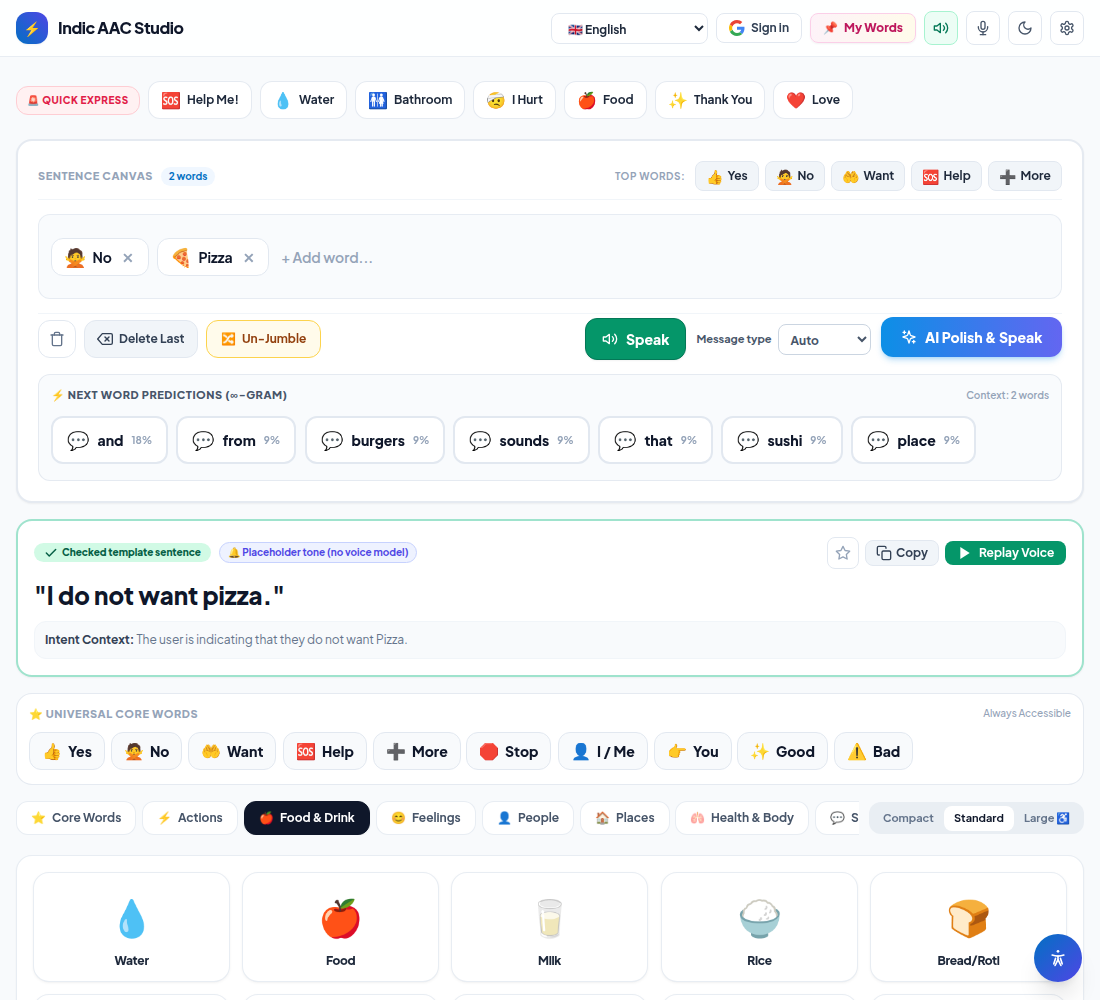
\includegraphics[width=\columnwidth,trim=20bp 340bp 640bp 510bp,clip]{figures/ui_fallback.png}\\[4pt]
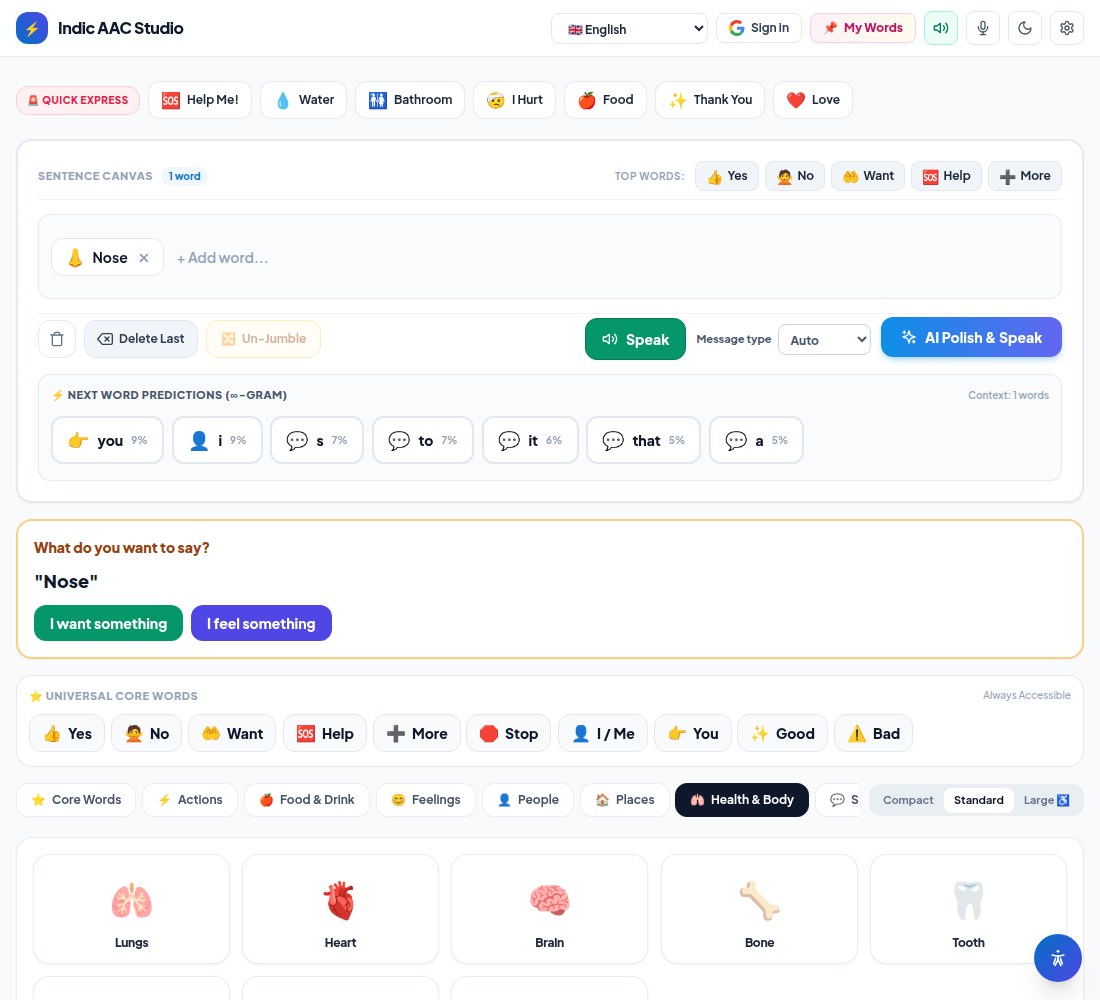
\includegraphics[width=\columnwidth,trim=20bp 340bp 640bp 510bp,clip]{figures/ui_clarification.png}
\caption{Recorded revised interface: (top detail) a rejected candidate leads to a labelled checked-template output; (bottom detail) an ambiguous selection asks the user to choose an act. The captured build labels its unavailable speech output as a 440 Hz test tone.}
\label{fig:ui}
\end{figure}

Next-word suggestions use an unbounded-order suffix trie inspired by infini-gram \citep{liu2024infinigram}, with suffix backoff weight 0.4.
The deployed trie contains 15,505 English and Hindi AAC-dialogue sentences and permits contexts up to depth 181.
Only English and Hindi have evaluated predictors; Gujarati returns English suggestions and Marathi reuses the Hindi trie.
Optional hidden Markov model (HMM) predictors and word reordering lack the required checkpoints in the evaluated build.
They therefore contribute no evidence to the sentence-generation comparison.

The configured neural speech route is \emph{IndicF5}, with a 24\,kHz \emph{Vocos} vocoder and reference-audio conditioning \citep{ai4bharat2025indicf5,siuzdak2023vocos}.
The IndicF5 model card lists Hindi, Gujarati, and Marathi among 11 supported languages, but does not list English.
The implementation nevertheless selects an English reference for English and an Indic reference for the other three languages; this routing is not evidence of successful synthesis.
The audited machines lacked the gated IndicF5 weights, all measured playback was a 440 Hz test tone, and headless Chrome exposed no browser voices.
Accordingly, the verified scope of this paper is sentence generation and playback integration, rather than audible four-language speech.

\section{Evaluation and Error Analysis}
\label{sec:eval}
We first evaluate the archived web-client path and then use explicit gold fields as a controlled diagnostic.
A separate regression analysis concerns the revised policy.
The systems, scorers, and input conditions are kept distinct because changing a scorer can alter a count without changing any sentence.

\subsection{Archived protocol and scoring}
The archived set has 184 monolingual scenarios: 46 selections in each language, comprising ten object requests, ten refusals, eight feelings, eight negated feelings, six action--object selections, and four help or call selections.
Nine selections duplicate few-shot examples and are excluded from the primary analysis, leaving 175 scenarios: 46 English, 45 Hindi, 42 Gujarati, and 42 Marathi.
Eight Hinglish scenarios are exploratory and are not pooled with these counts.
The archived run used one NVIDIA GTX~1650 with 4\,GB memory.

The lexical scorer requires every selected concept, correct gold polarity and act, no detected unselected concept, and an on-task sentence in the target script.
Concept retention has a different denominator: 215 required content-concept instances, rather than 175 scenarios.
Wrong act, missing act, added content, and off-task flags can overlap.
An off-task refusal is a model declining to answer, such as “I cannot help with that”; a legitimate user refusal, such as “I do not want pizza,” is on-task.
Lexical success does not establish grammaticality, meaning in context, or usefulness to AAC users.

The comparison includes literal labels, one unconstrained prompt to the same model, the archived cascade candidate before checking, the deployed policy, and the matched template.
The candidate and final text come from the same recorded response, isolating the joint effect of the gate, retry, and fallback.
The unconstrained prompt requests one sentence without a ledger, examples, refinement, or verification, using greedy decoding with a 75-token output cap; its 8/175 score diagnoses that prompt, rather than all one-pass methods.
Paired pooled intervals resample 46 underlying selection groups across their language versions, using 10,000 bootstrap resamples.

\begin{table*}[t]
\centering\small
\setlength{\tabcolsep}{5pt}
\begin{tabular}{@{}L{5.8cm}ccccc@{}}
\toprule
System / condition & English & Hindi & Gujarati & Marathi & Pooled \\
\midrule
\multicolumn{6}{@{}l}{\textit{A. Archived web client; scorer v1}}\\
Unconstrained Qwen (diagnostic) & 2/46 & 1/45 & 4/42 & 1/42 & 8/175 \\
Cascade before checking & 3/46 & 24/45 & 20/42 & 18/42 & 65/175 \\
Gate + retry + fallback & 22/46 & 31/45 & 21/42 & 23/42 & 97/175 \\
Matched template baseline & 33/46 & 31/45 & 27/42 & 27/42 & 118/175 \\
\midrule
\multicolumn{6}{@{}l}{\textit{B. Archived explicit gold act and polarity; scorer v1}}\\
Cascade before checking & 5/46 & 26/45 & 16/42 & 24/42 & 71/175 \\
Gate + retry + fallback & 33/46 & 41/45 & 26/42 & 32/42 & 132/175 \\
Matched template baseline & 46/46 & 45/45 & 34/42 & 42/42 & 167/175 \\
\midrule
\multicolumn{6}{@{}l}{\textit{C. Revised browser path; scorer v2; regression only}}\\
Revised cascade before checking & 6/46 & 29/45 & 27/42 & 26/42 & 88/175 \\
Revised gate + retry + checked fallback & 46/46 & 45/45 & 42/42 & 42/42 & 175/175 \\
Repaired template baseline & 46/46 & 45/45 & 42/42 & 42/42 & 175/175 \\
\bottomrule
\end{tabular}
\caption{Scenario success as counts over the same 175 selections. Panels A and B reproduce the archived lexical scorer; panel C is a scorer-v2 regression comparison on scenarios that informed the repairs. Scores across scorers are not directly comparable. English is a language reference; Hindi, Gujarati, and Marathi evaluate language extensions. The template is the method baseline in every language.}
\label{tab:results}
\end{table*}


\subsection{Web-client results and gold-field diagnostic}
With actual browser-inferred fields, the deployed policy succeeds on 97/175 scenarios, versus 65/175 before checking and 118/175 for the template (Table~\ref{tab:results}, panel A).
The policy--cascade difference is +18.3 percentage points (95\% interval 11.9 to 25.2); the policy--template difference is $-12.0$ points ($-17.9$ to $-6.4$).
The deployed policy retains 215/215 selected concept instances and has no detected polarity error, but still has 54 wrong-act outputs, four outputs with added content, and ten off-task outputs.
These diagnostics explain why complete retention alone is insufficient.

Supplying gold act and polarity raises the same deployed policy to 132/175, versus 71/175 before checking and 167/175 for the template (panel B).
The joint policy effect is +34.9 points (26.7 to 43.4); the gold-field--browser gap is +20.0 points (12.0 to 28.7).
The ungated gold-field cascade has 36 polarity errors, whereas the deployed output has zero detected errors.
Nevertheless, 37/108 accepted model outputs and 6/67 template fallbacks fail the full archived scorer.
Checker acceptance is therefore not interchangeable with independent success.

\subsection{Multilingual failure mechanisms}
The browser diagnostic sends 27 of 32 isolated feeling selections as requests.
Here 32 means eight feeling symbols in four locales, before any prompt-overlap exclusion; it is not the 30 feeling scenarios remaining in the primary score table.
The substring negation rule also mislabels three of 276 isolated symbol--language selections, including English \emph{Nose} and Gujarati \gu{નાક}.
Separating concept identity, act, and polarity directly addresses this input-layer defect.

The failure analysis includes all three Indic languages.
Recorded \lang{Hindi} feeling outputs include \bad{\hi{मुझे गुस्सा चाहिए।}} (\emph{“I want anger”}), where an intended state is realized as a request.
For \lang{Gujarati}, the eight apparent gold-field template failures are negated feelings with \gu{નથી}; the archived scorer omits this valid negator in its feeling-pattern test.
They are scorer lexical gaps, rather than evidence that these eight templates are wrong.
A recorded \lang{Marathi} tiredness output, \bad{\hi{मला दमलेला हवे आहे.}}, uses the request predicate \hi{हवे आहे} for an intended feeling; the archived scorer flags the act mismatch.
The checker must address act, perspective, and additions in each language; transferring English patterns alone does not do so.

The audit classifies the 37 accepted-model failures under gold fields as nine third-person reports, 12 negated-want constructions for feelings, ten malformed constructions, four additions, and two scorer gaps.
The six fallback failures are also scorer gaps.
These are assistant-produced diagnostic labels, not native-speaker judgments.
In particular, the lexical scorer's coverage affects both error counts and baseline rankings.

\subsection{Revised policy: regression evidence}
The repairs replace label-substring inference with concept-aware interpretation, add multilingual act and perspective checks, and check the fallback before returning it.
The same 175 scenarios informed these repairs and are therefore a regression set.
Under scorer v2, the archived policy scores 95/175 with browser fields and 138/175 with gold fields; the archived gold-field template scores 175/175 after its lexical gaps are corrected.
These are rescored archived sentences, not a new run of the old model.

The revised browser path and repaired template both score 175/175 on this set (Table~\ref{tab:results}, panel C).
The revised cascade alone scores 88/175, yielding a joint policy gain of 49.7 points (42.3 to 57.1).
This is a measured regression result, not evidence of generalization or superiority over the template.
A fresh 120-scenario set and blind rating materials exist, but native-speaker confirmation of their gold annotations and ratings are incomplete; we report no holdout performance or preference claim.
Figure~\ref{fig:workflow} and Table~\ref{tab:cases} show representative recorded cases rather than selecting only passing outputs.

\begin{table}[t]
\centering\footnotesize
\setlength{\tabcolsep}{2.8pt}
\begin{tabular}{@{}lrrrrrr@{}}
\toprule
&\multicolumn{3}{c}{English (reference)}&\multicolumn{3}{c}{Hindi}\\
\cmidrule(lr){2-4}\cmidrule(l){5-7}
Model & @1 & @5 & MRR & @1 & @5 & MRR \\
\midrule
Unigram & 3.6 & 11.6 & 0.069 & 6.4 & 14.5 & 0.099 \\
Bigram backoff & 13.6 & 29.5 & 0.204 & 24.0 & 43.1 & 0.320 \\
Trigram backoff & 16.0 & 32.8 & 0.234 & 25.9 & 44.0 & 0.334 \\
Suffix trie ($\infty$-gram) & 17.2 & 33.4 & 0.240 & 27.0 & 44.1 & 0.343 \\
Gutenberg HMM & 6.7 & 15.5 & 0.105 & -- & -- & -- \\
Hindi AAC HMM & -- & -- & -- & 24.5 & 41.9 & 0.315 \\
\midrule
\multicolumn{7}{@{}l}{Gujarati: no matched evaluation; shelf returns English.}\\
\multicolumn{7}{@{}l}{Marathi: no matched evaluation; reuses Hindi predictor.}\\
\bottomrule
\end{tabular}
\caption{Next-word prediction on AAC-user utterances from 60 of 300 source conversations per evaluated language (240 training; every fifth source held out). There are 2,220 English and 2,437 Hindi prediction contexts. Hit@1 and hit@5 are percentages; MRR is truncated at rank 10. Unigram is the frequency baseline. Dashes denote unmeasured cells, not zero performance.}
\label{tab:pred}
\end{table}


\subsection{Next-word prediction}
Table~\ref{tab:pred} evaluates AAC-user utterances in 60 held-out source conversations per evaluated language, not 60 utterances out of an unspecified pool.
Each language has 300 source conversations: 240 for training and 60 for testing, with every fifth source held out and no separate validation split in this evaluation.
All n-gram baselines and the evaluated suffix trie are rebuilt on the same 240 training sources, separately from the full-data deployed predictor.
Compared with trigram backoff, the trie gains 25/2,220 English and 29/2,437 Hindi hit@1 predictions: +1.126 points (95\% interval 0.505 to 1.766) and +1.190 points (0.463 to 1.922), computed from unrounded counts.
The corresponding hit@5 gains are 13/2,220 (+0.586 points) and 2/2,437 (+0.082 points).

Source conversations are disjoint, but 18 of 392 distinct English and 28 of 384 Hindi test utterances repeat training text.
Removing contexts from repeated utterances leaves 2,170 English and 2,352 Hindi contexts; trie--trigram hit@1 gains remain +0.968 and +1.020 points.
Out-of-vocabulary targets count as misses.
Gujarati and Marathi have no matched AAC prediction evaluation, so Table~\ref{tab:pred} records their coverage without inventing scores or treating language identity as a baseline method.

\subsection{Runtime and reproduction scope}
The revised browser-to-playback audit contains 32 runs across four languages, with one cold and 31 warm runs, on the GTX~1650.
Median click-to-first-playback is 9.9\,s and the 95th percentile is 20.8\,s; language medians are 12.4\,s (English), 15.3\,s (Hindi), 7.9\,s (Gujarati), and 10.7\,s (Marathi).
Every run plays a 440 Hz test tone: these are playback-integration timings, not click-to-audible-speech latency.
Greedy Indic retries repeated their first candidates in 40/40 uncached audit repeats, so the retry can add delay without changing the answer.

A CPU-only installation check reused cached weights; first-time download, clean GPU installation, and real synthesis were untested.
The model executes on the backend, but the browser requires externally hosted interface libraries and therefore is not verified as offline-ready.
No accessible public package or demo-video link was verified in the audit.

\section{Limitations and Conclusion}
\label{sec:limits}
The evidence comes from a small synthetic selection grid and a project-developed lexical scorer.
Native-speaker judgments and AAC-user studies have not established meaning preservation, naturalness, communication speed, or preference.
The repairs used regression scenarios; perfect scores do not establish semantic safety.
Gujarati and Marathi prediction, real speech, first-time installation, and offline operation remain unverified.
Native review, word-sense disambiguation, and complex negation scope are unresolved.

\paragraph{Availability and license.}
Local reproduction materials include scenarios, recorded candidates, scorers, repairs, and analysis procedures.
Public access and release licences for project code, dialogue data, manuscript figures, and demo media were not established.
Third-party terms remain Apache-2.0 for Qwen, MIT for IndicF5 and Vocos, and SIL OFL for Noto fonts.
Voice conditioning requires permission for the reference voice.

\paragraph{Conclusion.}
\sys{} makes concept, polarity, act checks, and fallback explicit for four-language symbol-to-sentence generation.
The archived policy improves its ungated cascade while trailing a matched template; the audit identifies defects in input interpretation, multilingual checks, and scoring.
The revised policy checks templates and offers clarification or literal preview.
Its regression result supports these repairs, while the value of model phrasing beyond templates remains unmeasured.

\section*{Acknowledgments}
Generative AI assistants Claude (Anthropic), ChatGPT, and Codex (OpenAI) assisted system merging, evaluation, scoring, manuscript revision, figures, and examples.
GPT-4o-mini generated the AAC dialogues; OPUS-MT English--Hindi translated the Hindi data.
Numerical statements trace to recorded results; these tools do not replace native-language review.

\section*{Ethics Statement}
An AAC system can misattribute needs, feelings, or consent to its user.
The interface should expose returned text and its route, preserve user control, and avoid automatically speaking ambiguous or unchecked content.
Neither a lexical score nor a checker verdict is a clinical safety certificate.
No AAC users or native raters participated in the reported results; the prepared rating materials do not constitute a completed study.
Future participant studies require appropriate consent, review, and accessible procedures.
Reference voices must be used only with explicit permission, and recordings or personal vocabulary should not be released without consent.

\bibliography{references}
\begin{figure*}[t]
\centering
\begingroup\footnotesize
\setlength{\tabcolsep}{4pt}\renewcommand{\arraystretch}{1.15}
\begin{tabular}{@{}L{1.3cm}L{2.1cm}L{4.0cm}L{2.8cm}L{3.9cm}@{}}
\toprule
Language & 1. Selection & 2. First candidate & 3. Check / route & 4. Returned text \\
\midrule
\multicolumn{5}{@{}l}{\textbf{A. Water request (positive polarity)}}\\
English\newline\textit{reference} & Water & I need \bad{food}.\newline\bad{[added: food; water missing]} & Reject: concept mismatch; checked template & \kept{I want water.} \\
Hindi\newline\textit{extension} & \hi{पानी} & \good{\hi{मुझे पानी चाहिए।}} & Pass; model text & \kept{\hi{मुझे पानी चाहिए।}} \\
Gujarati\newline\textit{extension} & \gu{પાણી} & \good{\gu{મને પાણી જોઈએ છે.}} & Pass; model text & \kept{\gu{મને પાણી જોઈએ છે.}} \\
Marathi\newline\textit{extension} & \hi{पाणी} & \good{\hi{मला पाणी हवे आहे.}} & Pass; model text & \kept{\hi{मला पाणी हवे आहे.}} \\
\midrule
\multicolumn{5}{@{}l}{\textbf{B. Pizza refusal (negative polarity)}}\\
English\newline\textit{reference} & No + Pizza & I cannot \bad{eat out} because I am .\newline\bad{[added: action/reason; pizza missing]} & Reject: concept mismatch; checked template & \kept{I do not want pizza.} \\
Hindi\newline\textit{extension} & \hi{नहीं + पिज़्ज़ा} & \good{\hi{पिज़्ज़ा, मुझे चाहिए।}} & Reject: negation missing; checked template & \kept{\hi{मुझे पिज़्ज़ा नहीं चाहिए।}} \\
Gujarati\newline\textit{extension} & \gu{ના + પિઝા} & \good{\gu{મને પિઝા નથી જોઈતું.}} & Pass; model text & \kept{\gu{મને પિઝા નથી જોઈતું.}} \\
Marathi\newline\textit{extension} & \hi{नाही + पिझ्झा} & \good{\hi{मला पिझ्झा हवे आहे.}} & Reject: negation missing; checked template & \kept{\hi{मला पिझ्झा नको आहे.}} \\
\bottomrule
\end{tabular}
\endgroup

\caption{Phase-wise recorded regression traces for all languages. Phase 1 supplies symbols and act/polarity, phase 2 proposes a candidate, phase 3 checks it (and retries if rejected), and phase 4 returns model or checked-template text. Panel A intends \emph{“I want water”}; panel B intends \emph{“I do not want pizza.”} Outputs are reproduced verbatim, including Gujarati agreement. “Pass” means checker acceptance, not native-judged correctness. English provides a reference-language row; Hindi, Gujarati, and Marathi are the proposed language extensions.}
\label{fig:workflow}
\end{figure*}

\newpage
\appendix
\section{Four-Language Interaction Traces}
\label{app:trace}
Figure~\ref{fig:workflow} follows the same two selections through all four phases in English and each Indic extension.
English is a language reference, not a competing system: every row uses the revised hybrid, the same model, and the same decision policy.
All candidate and returned strings are recorded regression outputs; green or blue text marks retained examples, and red marks a labelled unsupported addition.
Missing negation or a missing concept is stated explicitly because absent words cannot be highlighted.



\section{Representative Test Cases and Scorer Scope}
\label{app:scorer}
Table~\ref{tab:cases} samples every family in the six-family archived evaluation rather than listing every item.
The complete recorded scenario grid remains the denominator for reported results.
These cases additionally expose model acceptance, rejected candidates, checked fallbacks, and a limitation of lexical evaluation.
The corresponding phase-wise selections and outputs in Figure~\ref{fig:workflow} are a qualitative comparison, not evidence that one language performs better than another.

\begin{table*}[t]
\centering\footnotesize
\setlength{\tabcolsep}{4pt}\renewcommand{\arraystretch}{1.13}
\begin{tabular}{@{}L{2.7cm}L{3.7cm}L{8.5cm}@{}}
\toprule
Selection / intended act & English returned text & Indic selections $\longrightarrow$ returned text \\
\midrule
Water / request & \good{I want water.} & \textbf{HI} \hi{पानी} $\rightarrow$ \good{\hi{मुझे पानी चाहिए।}}\newline \textbf{GU} \gu{પાણી} $\rightarrow$ \good{\gu{મને પાણી જોઈએ છે.}}\newline \textbf{MR} \hi{पाणी} $\rightarrow$ \good{\hi{मला पाणी हवे आहे.}} \\
No + Pizza / refusal & \good{I do not want pizza.} & \textbf{HI} \hi{नहीं + पिज़्ज़ा} $\rightarrow$ \good{\hi{मुझे पिज़्ज़ा नहीं चाहिए।}}\newline \textbf{GU} \gu{ના + પિઝા} $\rightarrow$ \good{\gu{મને પિઝા નથી જોઈતું.}}\newline \textbf{MR} \hi{नाही + पिझ्झा} $\rightarrow$ \good{\hi{मला पिझ्झा नको आहे.}} \\
Tired / feeling & \good{I am tired.} & \textbf{HI} \hi{थका हुआ} $\rightarrow$ \good{\hi{मैं थका हुआ हूँ।}}\newline \textbf{GU} \gu{થાકેલું} $\rightarrow$ \good{\gu{હું થાકેલું છું.}}\newline \textbf{MR} \hi{दमलेला} $\rightarrow$ \good{\hi{मी दमलेला सांगत आहे.}} \\
No + Happy / negated feeling & \good{I am not happy.} & \textbf{HI} \hi{नहीं + खुश} $\rightarrow$ \good{\hi{मैं खुश नहीं हूँ।}}\newline \textbf{GU} \gu{ના + ખુશ} $\rightarrow$ \good{\gu{હું ખુશ નથી.}}\newline \textbf{MR} \hi{नाही + आनंदी} $\rightarrow$ \good{\hi{मी आनंदी नाही.}} \\
Drink + Water / action request & \good{I want to drink water.} & \textbf{HI} \hi{पीना + पानी} $\rightarrow$ \good{\hi{पीना, मुझे पानी चाहिए।}}\newline \textbf{GU} \gu{પીવું + પાણી} $\rightarrow$ \good{\gu{મને પાણી પીવાનું મન છે.}}\newline \textbf{MR} \hi{पिणे + पाणी} $\rightarrow$ \good{\hi{मला पाणी पिण्याची इच्छा आहे.}} \\
Call + Mother / call request & \good{I want to call my mother.} & \textbf{HI} \hi{फ़ोन करना + माँ} $\rightarrow$ \good{\hi{माँ, मुझे फ़ोन करना हूँ, मुझे चाहिए।}}\newline \textbf{GU} \gu{ફોન કરવો + માતા} $\rightarrow$ \good{\gu{મને માતાને ફોન કરવાનું મન છે.}}\newline \textbf{MR} \hi{फोन करणे + आई} $\rightarrow$ \good{\hi{मला आईला फोन करण्याची इच्छा आहे.}} \\
\bottomrule
\end{tabular}
\caption{Representative recorded revised-browser regression cases: one underlying message per archived family, shown in all four languages. HI: Hindi; GU: Gujarati; MR: Marathi. Act and polarity are supplied separately from the visible labels. These are exact system outputs, including awkward accepted constructions (e.g., the Marathi tiredness report and Hindi call request). Colour indicates an example, not human validation.}
\label{tab:cases}
\end{table*}


The archived scorer defines off-task behavior through refusal-to-answer patterns, third-person narration, empty output, length over 25 whitespace tokens, and Latin leakage in an Indic target.
It can confuse a missing pattern with an error, as the Gujarati negated-feeling audit demonstrates.
The revised scorer broadens lexical forms and separates perspective, polarity, act, and additional concepts.
It is still not a native-speaker assessor, and scorer-v1 and scorer-v2 success totals must not be merged.

\section{Reproduction and Language Coverage}
\label{app:models}
The prompted model is \model{}, revision 7ae557604adf67be50417f59c2c2f167def9a775.
It is used as released, without task-specific fine-tuning, with 16-bit floating-point inference on GPU.
Archived generation ran on a GTX~1650 (4\,GB); revised regression generation ran on a TITAN~Xp (12\,GB) with PyTorch 2.11.0 and Transformers 5.14.1.
English regression sampling uses seed 11; the three Indic paths are greedy.
The complete saved stream, rather than a selectively regenerated candidate, is replayed for each paired policy comparison.

The predictor split has 240 training and 60 test source conversations per evaluated language (300 in total; no separate validation split).
Each target is a next word from an AAC-user utterance; source-conversation bootstrap intervals keep its contexts together.
HMM baselines in Table~\ref{tab:pred} are separate prediction components, not the sentence realizer.
Gujarati and Marathi text-generation coverage therefore does not imply evaluated next-word prediction or verified speech coverage.

Clarification is tested separately from sentence success.
In the recorded user-choice probe, the user selects an act for an ambiguous word before the system continues; the act choice can still lead to a lexical match with the wrong sense.
For example, a Gujarati feeling interpretation of an ambiguous label yields \gu{હું ખરાબ છું.}, which can mean \emph{“I am bad”} rather than feeling unwell.
The gate's lexical match does not settle that distinction.
An unavailable server yields a labelled literal preview; no candidate is invented to fill that failure.

\end{document}
